\subsection{Struktura}\label{subsec:struktura}
W sumie przeanalizowanych zostało 135 zestawów danych.
Pojedynczy zestaw danych składa się z pomiarów czujników rozmieszczonych w różnych miejscach na pojedynczym obiekcie.
Liczba czujników waha się od kilku do kilkudziesięciu.
Każdy czujnik jest scharakteryzowany przez następujące dane:
\begin{itemize}
    \item identyfikator,
    \item odległość bazowa — oznaczająca odległość zmierzoną przez laserowe urządzenie pomiarowe, w chwili uruchomienia monitoringu na obiekcie,
    \item seria pomiarów — notująca odległość czujnika od podłoża w kolejnych momentach.
\end{itemize}
Rozwiązanie zostało opracowane na podstawie pomiarów 1225 urządzeń i około 600 tys.\ pomiarów odległości.

\subsection{Charakterystyka}\label{subsec:charakterystyka}

\subsubsection{Odstępy czasu}
\begin{figure}[h]
    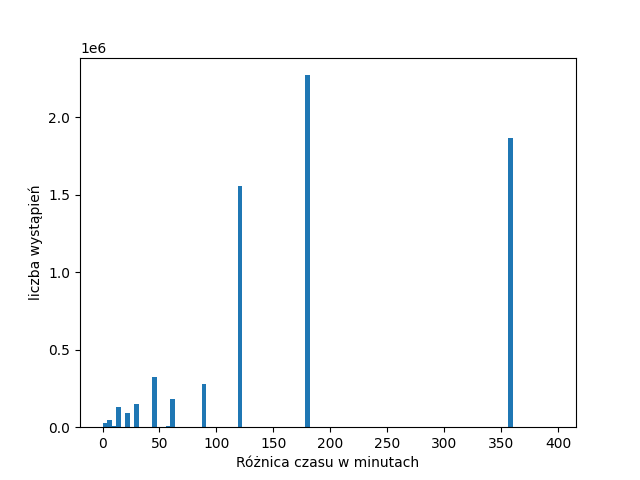
\includegraphics[width=\textwidth]{time_diff.png}
    \caption{Zbiorczy histogram przedstawiający odstępy czasu między kolejnymi pomiarami dla wszystkich danych.}\label{fig:odstepyczasu}
\end{figure}

Rysunek~\ref{fig:odstepyczasu} pokazuje, że przez większość czasu okres raportowania wynosi 2,3 lub 6 godzin.
By ułatwić komputerową analizę, dane zostały przepróbkowane do okresu 3h.
Finalnie, każdy okres jest reprezentowany przez jedną wartość pomiaru.
Każdy przedziały czasu z co najmniej jednym pomiarem jest zagregowany do mediany.
Każdy przedział 3-godzinny bez żadnego pomiaru jest reprezentowane przez ostatni pomiar przed tym przedziałem.

Mediana jest tutaj właściwym agregatorem, ponieważ jest ona odporna na duże odchylenia, w przeciwieństwie do np.\ średniej.

\subsubsection{Różnice odległości}
\begin{figure}[h]
    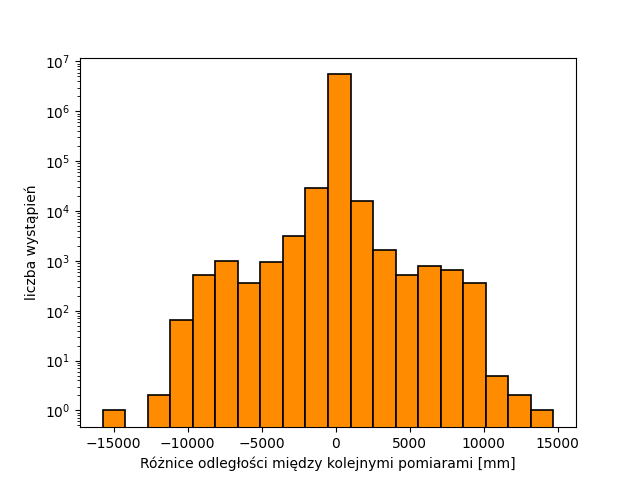
\includegraphics[width=\textwidth]{dist_diff_big.png}\caption{Zbiorczy histogram różnic między kolejnymi pomiarów odległości dla wszystkich danych przed przepróbkowaniem.}
    \label{fig:distbig}
\end{figure}

Bardzo istotne jest to, że na rysunku~\ref{fig:distbig} pionowa skala jest logarytmiczna.
Z informacji dostarczonych przez firmę wiadomo, że wychylenia w ciągu kilku godzin mogą być co najwyżej 25-milimetrowe.
Ta informacja pokrywa się z wyżej pokazanym wykresem.
Można zaobserwować strzeliste rozkłady normalne dużych zastawień po bokach ze środkiem na poziomie 7 metrów.
Bardzo wysoki szpic do 25 milimetrów reprezentuje zdecydowaną większość obserwacji, co widać na rysunku~\ref{fig:diffsmall}.


\begin{figure}[h]
    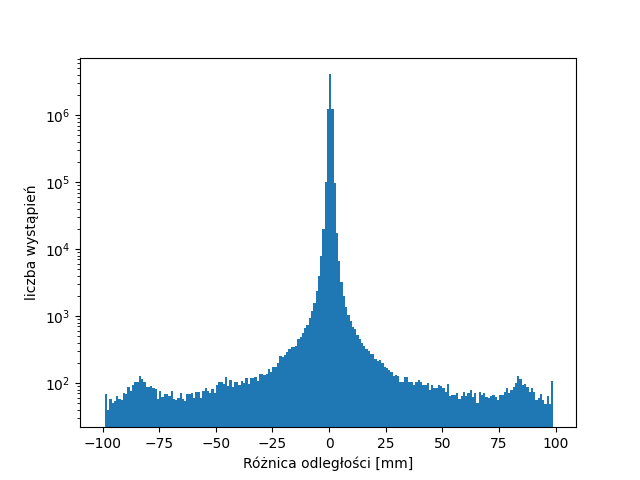
\includegraphics[width=\textwidth]{dist_diff_small.png}
    \caption{Zbiorczy histogram różnic między kolejnymi pomiarów odległości dla wszystkich danych obcięty do 100 mm.}
    \label{fig:diffsmall}
\end{figure}


Po przepróbkowaniu rozkład pozostał bez większych zmian, co można zaobserwować na rysunku~\ref{fig:diffsmallresampled}.
\begin{figure}[h]
    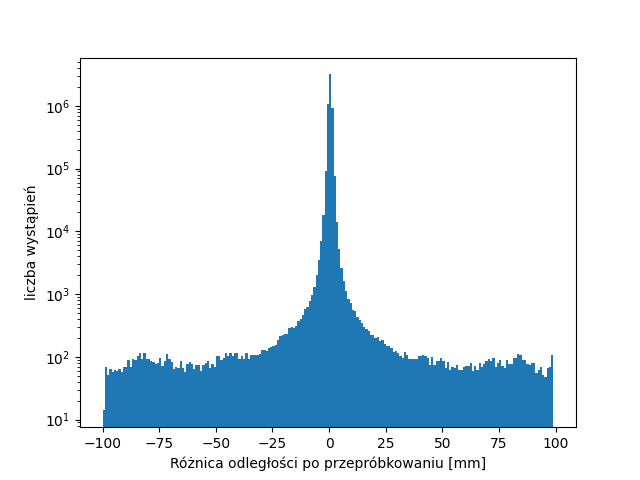
\includegraphics[width=\textwidth]{dist_diff_small_resampled.png}
    \caption{Zbiorczy histogram różnic między kolejnymi pomiarów odległości dla wszystkich danych, po przepróbkowaniu do okresów 3-godzinnych, obcięty do 100 mm.}
    \label{fig:diffsmallresampled}
\end{figure}


\subsubsection{Różnice bazy od odległości}
\begin{figure}[h]
    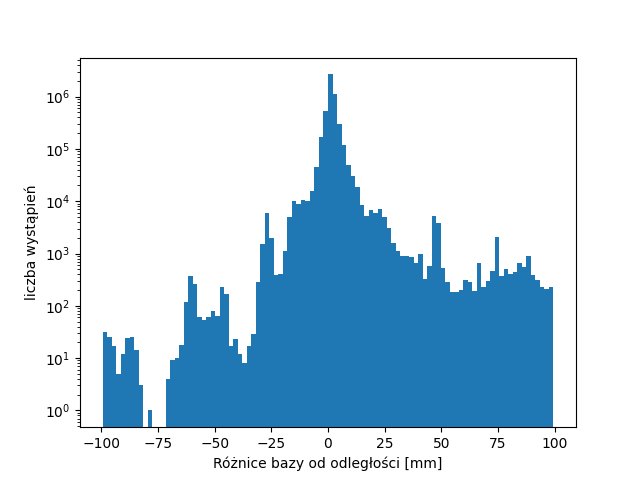
\includegraphics[width=\textwidth]{dist.png}
    \caption{Zbiorczy histogram różnic odległości bazowej od pomiarów odległości.}
    \label{fig:dist}
\end{figure}


Dane na rysunku~\ref{fig:dist} są ponownie przedstawione w skali logarytmicznej, bo w przeciwnym wypadku nie dałoby się niczego zauważyć.
Zdecydowana większość obserwacji oscyluje wokół zera.
Mediana jest równa zero.
Będzie to kluczowe — prawdziwe ugięcia dachu powinny być krótkotrwałe i w dłuższej perspektywie mediana pomiarów powinna wynosić zero.
\subsubsection{Przykłady danych}\label{examples}
Górne części wykresów reprezentują wszystkie pomiary, a dolne obcięte do maksymalnie 25 mm wychylenia.

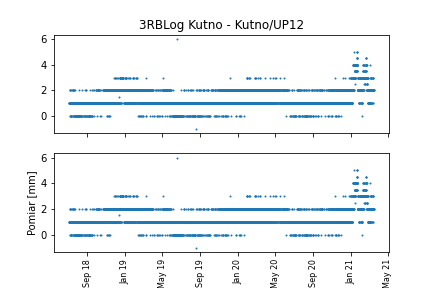
\includegraphics[width=0.9\textwidth]{example11.png}

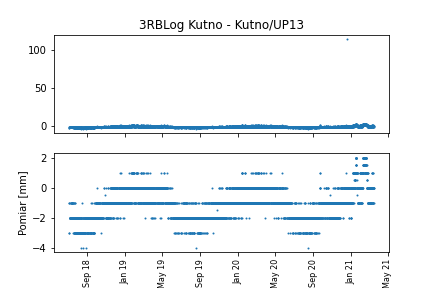
\includegraphics[width=0.9\textwidth]{example12.png}

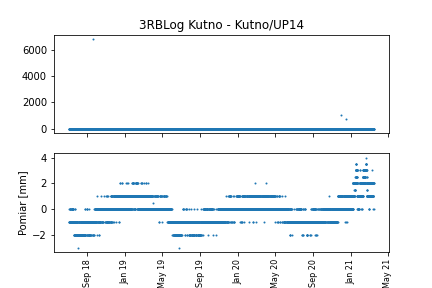
\includegraphics[width=0.9\textwidth]{example13.png}

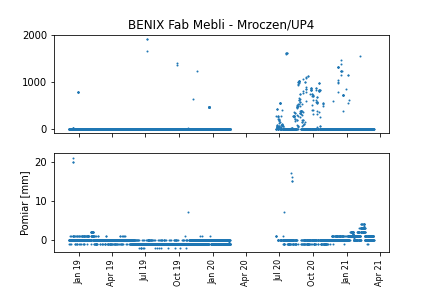
\includegraphics[width=0.9\textwidth]{example50.png}

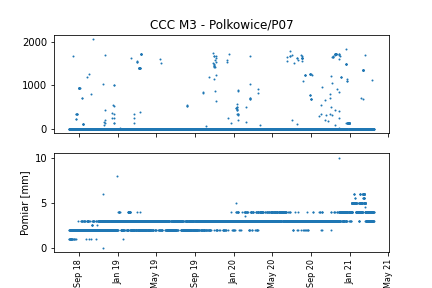
\includegraphics[width=0.9\textwidth]{example400.png}\phantomsection\label{mroczen}

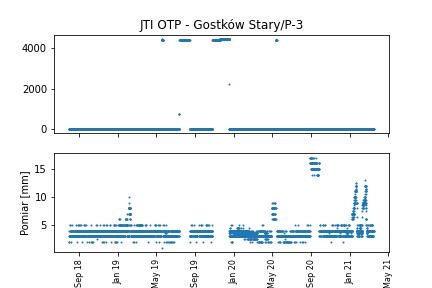
\includegraphics[width=0.9\textwidth]{example812.png}\phantomsection\label{jti}

\subsubsection{Autokorelacja}\label{autocorrelation}

Na rysunku~\ref{fig:autocorrelation} pokazana jest zbiorcza autokorelacja wszystkich szeregów czasowych, w zależności od przesunięcia.
Niebieskim cieniem jest zaznaczony przedział ufności (ang.\ \emph{confidence interval}).
\begin{figure}[h]
    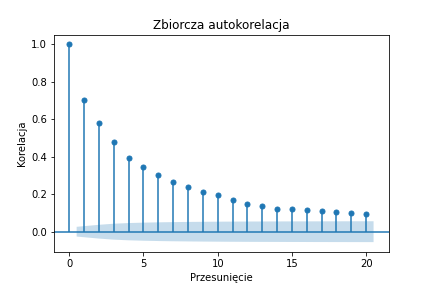
\includegraphics[width=0.9\textwidth]{autocorrelation.png}
    \caption{Zbiorcza autokorelacja różnicy odległości bazowej od pomiaru dla wszystkich zestawów danych.}
    \label{fig:autocorrelation}
\end{figure}

\subsubsection{Podsumowanie}
Na przykładzie pierwszych trzech urządzeń z sekcji~\ref{examples}, widzimy, że odgięcia dachu w tym samym obiekcie mogą być wysoce skorelowane.
Dane z urządzenia \hyperref[mroczen]{BENIX Fab Mebli - Mroczen/UP4} pokazują, że zastawienia mogą występować nawet po odcięciu danych powyżej 25 mm.
Dane z urządzenia \hyperref[jti]{JTI OTP - Gostków Stary/P-3} pokazują oczywiste zastawienie na poziomie 15 mm — wysokość położonej paczki papierosów.

Autokorelacja jest na tyle statystycznie istotna, że jesteśmy w stanie dosyć dobrze zamodelować nasz szereg czasowy autoregresją z oknem o długości 20.
